\documentclass[12pt,spanish,letterpaper,color]{uchile}
\usepackage{ucs}
\usepackage[utf8x]{inputenc}
\usepackage[spanish]{babel}
\PrerenderUnicode{áéíóúÁÉÍÓÚüÜ}
%%%%%%%%%%%%%%%%%%%%%%
%% Para macros propias
\usepackage{xspace}

%move to class?
%%usa punto en vez de coma en las ecuaciones con decimales, tiene que ir despues de babel
\decimalpoint
%%%%%%%%%%%%%%%%%%%%%%
%% Mathematical packages
\usepackage{amsmath}
\usepackage{amsthm}
\usepackage{amssymb}

%move to class?
%%  paquete para setear los margenes, verificar
\usepackage[right=2cm,left=3cm,top=2cm,bottom=2cm,headsep=0cm,footskip=1cm]{geometry}
%\usepackage{anysize}
%\papersize{27.94cm}{21.59cm}
%\marginsize{3.0cm}{2.0cm}{2.0cm}{2.0cm}


%move to class?
%% paquete para insertar links en pdf
%colorlinks=true, resalta los links con colores
\usepackage[pdftex,pdfborderstyle={/S/U/W 0}, 
pdftitle={Memoria}, 
pdfauthor={Felipe Lema}, 
pdfsubject={Emulación}, pdfkeywords={p2p, kaillera, emulación},
pdfcreator={Felipe Lema}]{hyperref}

%%%%%%%%%%%%%%%%%%%%%%
%% Cite Package
%% must go after hyperref
%% debe ir depues de hyperref
\usepackage{cite}

%%%%%%%%%%%%%%%%%%%%%%
%% Numprint Pacakge
%% allows to print number with automatic thousand separator and decimal separator
%% Ejxamples: \numprint{2006.3}-> 2.006,3 \numprint{20009}-> 20.009
%% permite escribir numeros con separador de miles y con separador decimal. 
%% Ejemplos: \numprint{2006.3}-> 2.006,3 \numprint{20009}-> 20.009
\usepackage[autolanguage]{numprint}
\npthousandsep{.}\npdecimalsign{,}

\newtheorem{lemma}{Lema}%we can specify the counter in brackets
\newtheorem{corollary}{Corolario}
\newtheorem{theorem}{Teorema}
%\renewcommand{\bibliographyname}{Bibliografía u otro nombre}
%%%%%%%%%%%%%%%%%%%%%%
%% Listings Package
%% Printing program/source code (C++ code)
%% Imprime código fuente/ de programa (código C++)
\usepackage{listings}
\usepackage{color}
\definecolor{gray97}{gray}{.97}
\definecolor{gray75}{gray}{.75}
\definecolor{gray45}{gray}{.45}

\lstset{ frame=Ltb,
     framerule=0pt,
     aboveskip=0.5cm,
     framextopmargin=3pt,
     framexbottommargin=3pt,
     framexleftmargin=0.4cm,
     framesep=0pt,
     rulesep=.4pt,
     backgroundcolor=\color{gray97},
     rulesepcolor=\color{black},
     %
     stringstyle=\ttfamily,
     showstringspaces = false,
     basicstyle={\ttfamily\small},
     commentstyle=\color{gray45},
     keywordstyle=\bfseries,
     %
     numbers=left,
     numbersep=15pt,
     numberstyle=\tiny,
     numberfirstline = false,
     breaklines=true,
     %
     float,
     language=C++,
     columns=fixed,
     escapeinside={//*}{\^^M}, %labels
     tabsize=2
   }
\renewcommand{\lstlistlistingname}{Códigos}
\renewcommand{\lstlistingname}{Código}

%%%%%%%%%%%%%%%%%%%%%%
%% Algorithms Package
%% Printing pseudocode
%% Imprime pseudo-código
\usepackage{algorithmic}


%%%%%%%%%%%%%%%%%%%%%%
%% clrscode3e Package
%% Typeset pseudo-code "Intro to Algorithms" style
%% Formatea pseudo-código al estilo de "Introducción a Algoritmos"
\usepackage{clrscode3e}

%%%%%%%%%%%%%%%%%%%%%%
%% subfig Package
%% to have subfigures within figures, or subtables within table floats
\usepackage{subfig}

\begin{document}
%%%%%%%%%%%%%%%%%%%%
%macros
%%%%%%%%%%%%%%%%%%%%
\newcommand{\kai}{\textit{Kaillera}\xspace}
\newcommand{\fba}{\texttt{fba}\xspace}


%%%%%%%%%%%%%%%%%%%%
%Definicion de variables de la portada
%%%%%%%%%%%%%%%%%%%%
%%Logo
%\grafica{escudocolor.png}{Logo de la Universidad de Chile}{logo}{0.6}
%% B. Nombre Institucion
\universidad{Universidad de Chile}
\facultad{Facultad de Ciencias Físicas y Matemáticas}
\departamento{Departamento de Ciencias de la Computación}
%% C. Titulo
\title{Autenticación Desmentible en Canales Anónimos}
%% D. Proposito titulacion
\trabajoygrado{Presentación del Tema de Memoria para optar al título de Ingeniero Civil en Computación}
%% E. Autor
\author{Alonso Emilio González Ulloa}
%% F. Profesores guia, co-guia e integrantes, los 3 primeros son obligatorios
\profguia{Alejandro Hevia Angulo} %profesor guia
\profcoguia{Gonzalo Navarro Badino} %profesor co-guia
\profint{Rodrigo Paredes Moradela} %profesor integrante
%\profinta{Sr. ZZ ZZ ZZ} %profesor integrante 2, generalemente no es necesario
%\profintb{Sr. ZZZ ZZZ ZZZ} %profesor integrante 3, generalmente no es necesario
%% G. Lugar y fecha
\ciudad{Santiago}
\pais{Chile}
\monthpub{Marzo}
\yearpub{2011}
%por ahora hay que poner el proyecto en mayusculas y si los saltos de linea deben ir a mano
%\proyecto{ESTE TRABAJO HA SIDO FINANCIADO EN PARTE POR EL PROYECTO \\ FONDECYT 12345678 Y POR EL PROYECTO CORFO 2009/8956-4}

%%%%%%%%%%%%%%%%%%%%%
%% Lista de TODOS y FIXMEnS, no aparece si es que no hay nada que hacer
\listoftodos
\newpage
%% Portada
\maketitle

%% Pagina optativa, ahora creo que ya no va
%\section{Calificaciones}
%\makeeval
% Necesita revision en caso de uso
\begin{preface} 
%%%%%%%%%%%%%%%%%%%%%%%%%%%%%%
%% Resumen


%%%%%%%%%%%%%%%%%%%%%%%%%%%%
%% Dedicatoria: Pagina Optativa
%\dedicatoria{A mi Sol}
%% Pagina optativa
%%%%%%%%%%%%%%%%%%%%%%%%%%%%
%% Agradecimientos: Pagina Optativa
\section{Agradecimientos}
Agradezco a mi profesor guía Jo por su apoyo y orientación a lo largo de este trabajo. Nahid
Akbar (a.k.a. Killer Civilian) por sus opiniones y conociemientos con \kai \textit{p2p}.
\texttt{iq\_132} y los usuarios de los foros de FinalBurn Alpha por su ayuda con el código del
emulador. A Joaquín, Sebastián y Haníbal por sus \textit{feedbacks}.\\

%Finalmente, al buscador Google por responderme tan rápido las dudas técnicas para esta memoria.\\
\begin{flushright}
Felipe Lema S.
\end{flushright}
%%%%%%%%%%%%%%%%%%%%%%%%%%%%%%
%% Indices varios
%% Indice General
\tableofcontents
%% Indice de Tablas : Pagina Optativa
%\listoftables
%% Indice de Figuras : Pagina Optativa
\listoffigures

\end{preface}
%%%%%%%%%%%%%%%%%%%%%%%%%%%%%%

\chapter{Introducción}

\section{Motivación}
Para motivar el tema a tratar en este trabajo, presentamos el siguiente problema que
perfectamente se podría presentar en un escenario real.\\
El tribunal de la libre competencia (TDLC) desea desarrollar una plataforma que permita
a las distintas empresas presentar pruebas que inculpen
a otra empresa en delitos como colusión, monopolio, etc. Para ello pondrá
a disposición de las empresas un conjunto de servidores a los cuales enviar sus denuncias.\\
Para no amedrentar a una empresa
denunciante  es necesario que la comunicación entre la empresa y cada servidor
sea anónima. Pues de este modo ningún observador podría determinar que una empresa a denunciado
a otra de cierto delito y tomar represalias.\\
Por otro lado el TDLC confía más en el testimonio de algunas empresas que en el de otras, ya sea por
su conducta anterior u otros factores. Por lo tanto desea estar completamente seguro de la identidad
de una empresa cuando esta empresa presente pruebas usando la plataforma, pues así puede determinar
un factor de credibilidad en la denuncia.\\
La plataforma correrá en internet, por lo tanto debe mantener sus propiedades de seguridad inclusive
si es ejecutada concurrentemente con protocolos maliciosos.\\
Para desarrollar la plataforma el TDLC ha determinado que su problema es exactamente el siguiente:\\
\textit{Desea crear un protocolo mediante el cual las empresas se comuniquen con cada uno de los servidores
de denuncias. La comunicación entre empresas y servidores debe ser anónima y autentificada, y esto se
debe cumplir inclusive si el protocolo es ejecutado concurrentemente con otros protocolos.}\\ 

\section{Descripción del problema}

En general el problema anterior puede a aplicarse a cualquier de grupo de personas que
desea comunicarse entre sí en una red (internet o una red local) y desea obtener garantías
similares. A continuación iniciamos el camino de formalización del problema motivacional.\\
La solución del problema consiste en encontrar un protocolo (un algoritmo distribuido) de cual
se puedan garantizar matemáticamente las siguientes tres propiedades :
\begin{enumerate}
    \item Anonimato
    \item Autentificación desmentible
    \item Componibilidad
\end{enumerate}

\subsubsection{Anonimato}
A modo de ejemplo podemos considerar un protocolo ``usual" de comunicación, un protocolo IP simplificado.
En la figura \ref{tcpip_simple} cada flecha de $A$ a $B$ indica que $A$ envió un me saje a
$B$. La etiqueta de una flecha de $A$ a $B$ indica el mensaje intercambiado en la ejecución de protocolo.
Por ejemplo Empr-1 envió a Serv-1 el mensaje $(m_{e1s1}, ip_{e1}, ip_{s1})$, donde $m_{e1s1}$ es el contenido
del mensaje, $ip_{e1}$ es la dirección IP de la Empresa 1 e $ip_{s1}$ es la dirección IP del Servidor 1.
Notemos que estos
datos son necesarios para poder \textit{rutear} los mensajes de un participante a otro, pero a la vez 
se revela a un observador que Empr-1 envió un mensaje a Serv-1. Por lo tanto podemos decir que
\textbf{el protocolo IP simplificado no es anónimo} pues \textbf{existe un ataque}.\\

\begin{figure}[hp]
    \centering
    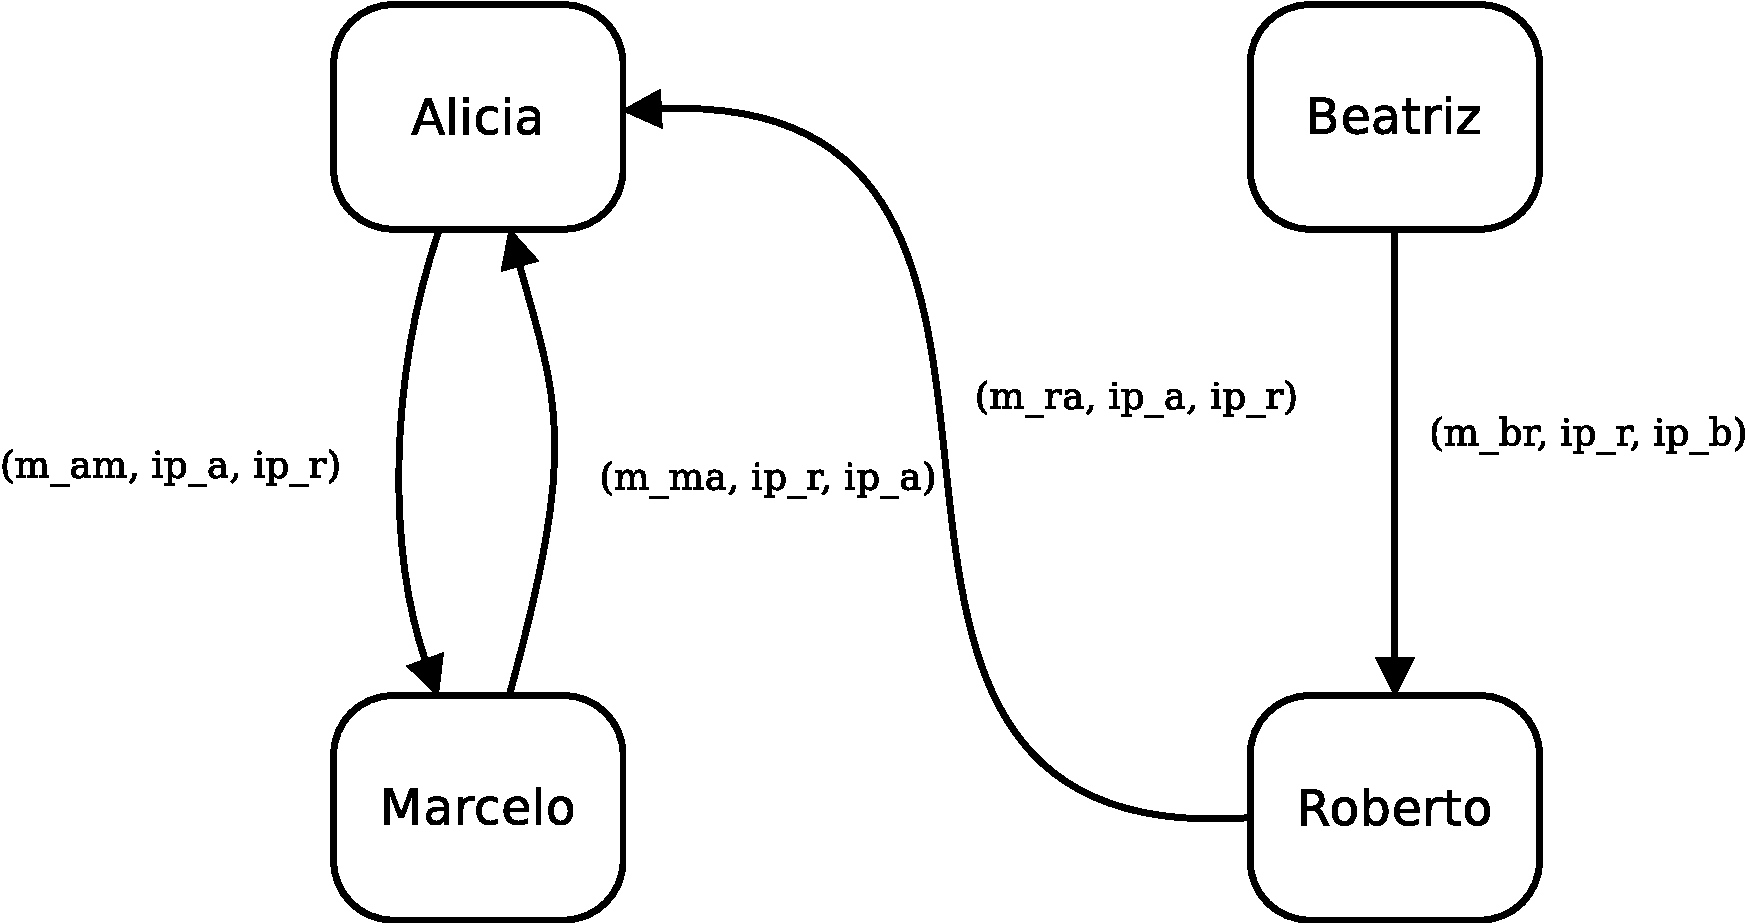
\includegraphics[width=0.7\textwidth]{figs/tcpip_simple}
    \caption{Protocolo simple de comunicación}
    \label{tcpip_simple}
\end{figure}

Para definir el anonimato resulta crucial definir formalmente que es considerado
un ataque al anonimato, pues un protocolo será anónimo si y solo si no existe ningún ataque.
En \cite{conf/pet/HeviaM08} se define un ataque con el siguiente juego.
El observador o adversario determinada dos posibles ejecuciones del protocolo, las cuales difieren en
qué mensajes serán enviados por quién y qué mensajes serán recibidos por quién. Entonces
consideraremos que el adversario realiza un ataque si al ejecutar al adversario con cada una
de las posibles ejecuciones del protocolo, el adversario logra identificar cuál es cuál.
Por lo tanto un protocolo sera seguro si y solo si cualquier adversario no logra distinguir
una ejecución de otra.

\subsubsection{Autentificación desmentible}
En el protocolo de la figura \ref{tcpip_simple} es posible que un adversario (rol que puede
asumir una empresa $Empr-2$) se haga pasar por una empresa $Empr-1$ con buena reputación y denuncie
falsamente a una empresa enemiga $Empr-3$. Para ello
solo es necesario que modifique uno de sus mensajes cambiando $ip_e2$ por $ip_e1$.
Por lo tanto decimos que el protocolo no implementa canales autenticados.\\
Con canales autentificado nos referimos protocolos en los cuales es posible estar seguro,
con alta probabilidad, de quién es el autor de un mensaje. Sin embargo hay que ser cuidadoso
con el protocolo de autentificación usado, pues los más conocidos
(firmas digitales por ejemplo) poseen la propiedad de \textit{non repudiability}. Esto es,
que el emisor de un mensaje autentificado no puede negar a ``la comunidad" que el es el autor
del mensaje. Esto estaría contradiciendo el anonimato, pues el adversario también sería capaz
de asociar la autoría de un mensaje a el emisor de este.\\
La autentificación desmentible, introducida en \cite{DwoNaoSah04}, se refiere a los protocolos
que implementan canales anónimos con la propiedad adicional de que cada mensaje es autentificado
a un receptor específico y el receptor no es capaz de probar a nadie más quién es el autor del mensaje.

\subsubsection{Componibilidad}
En general el hecho de implementar protocolos con ciertas garantías (por ejemplo anonimato y
autentificación desmentible) no garantiza que dichas propiedades se sigan teniendo cuando
el protocolo es ejecutado concurrentemente con otros protocolos.\\
En \cite{conf/focs/Canetti01} Canetti introduce el \textit{framework} criptográfico conocido
como \textit{Universal Composabillity} (desde ahora UC). UC propone una metodología definir y
demostrar los objetivos de seguridad de un protocolo (por ejemplo anonimato y autentificación)
de un protocolo. UC garantiza que el protocolo mantendrá su seguridad inclusive
si es ejecutado concurrentemente con cualquier protocolo, siempre y cuando no comparta estado
con el protocolo analizado.\\
Cuando el protocolo sí comparte estado con otros protocolo es necesario hacer uso del
\textit{framework Generalized Universal Composabillity} (desde ahora GUC), que generaliza a UC.
Informalmente GUC propone una metodología para incluir el estado que un protocolo podría compartir
con otros.

\section{Objetivos}

\subsection{Objetivo General}
Diseñar un protocolo criptográfico eficiente que cumpla nociones razonables
de Anonimato y Autentificación Desmentible. Demostrar matemáticamente su
seguridad usando herramientas modernas de análisis criptográficas (GUC), y
estudiar su relación con otras primitivas criptográficas.

\subsection{Objetivos específicos}

\begin{enumerate}
    \item Estudiar conceptos asociados a interacciones desmentibles y las técnicas y
          primitivas criptográficas asociadas (encriptación y mecanismos de autentificación
           como firmas digitales y esquemas de identificación).
    \item Estudiar conceptos de anonimato y las técnicas y primitivas criptográficas
          asociadas.
    \item Proponer un protocolo que combine ambas nociones.
    \item Analizar dicho protocolo en términos de efectividad y eficiencia.
    \item Analizar la efectividad en términos de las garantías de seguridad obtenidas.
    \item Analizar la eficiencia en términos de los costos en tiempo asociados al
          protocolo.
    \item Estudiar su relación con otros protocolos criptográficos.
\end{enumerate}


En la figura \ref{sigmix_simple} se muestra un diagrama para explicar nuestra solución.

\begin{figure}[hp]
    \centering
    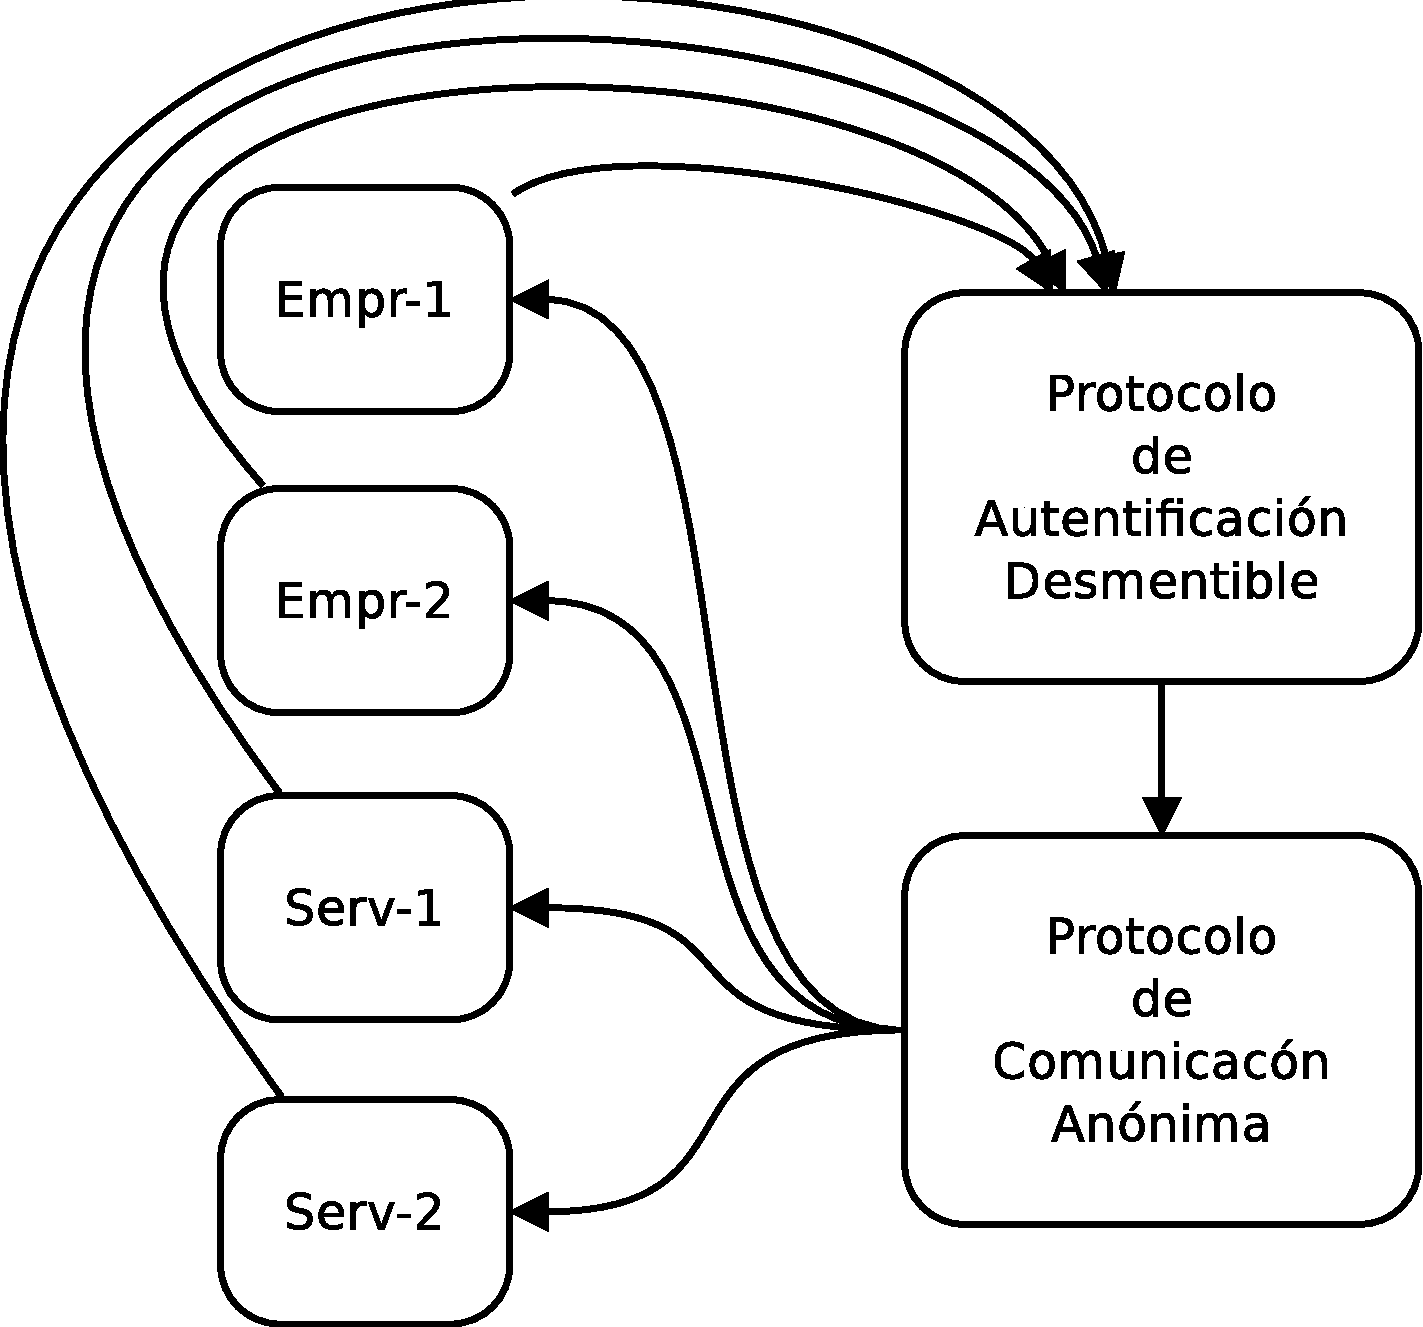
\includegraphics[width=0.5\textwidth]{figs/sigmix_simple}
    \caption{Solución propuesta}
    \label{sigmix_simple}
\end{figure}


%TODO Habrá un nombre mejor?
\chapter{Marco Teórico}

En este capítulo hacemos distintas definiciones básicas útiles
para este trabajo.

\section{Definiciones básicas}

\begin{definicion}[String]
Decimos que $\omega$ es un string si $\omega \in \{0,1\}^*$.
\end{definicion}

\begin{definicion}[Largo de un string]
Para un string $\omega$ denotamos por $|\omega|$ al entero $k$
tal que $k$ es el número de caracteres de $|\omega|$.
\end{definicion}

\begin{definicion}[Función despreciable]
Decimos que una función $\eta: \mathbb{N} \to \mathbb{N}$ es despreciable
si crece más lento que el inverso de cualquier polinomio. Es decir, para
todo polinomio $p$ existe
un $n_0$ talque para todo $n > n_0$ se cumple que
$$\eta(n) < \frac{1}{p(n)}$$
\end{definicion}
Las funciones despreciables permiten definir probabilidades ``pequeñas'' para cualquier
variable aleatoria ``algorítmica''. Es decir, variables aleatorias que corresponden a la
salida de un algoritmo.\\
Una forma de ver la utilidad de las funciones despreciables es la siguiente. Consideremos
el caso en que queremos determinar si un lenguaje $L$ es \textit{difícil}, esto es, para
cualquier algoritmo de tiempo polinomial determinar si $x \in L$ es difícil.
Diremos que un algorimo $A$ tiene éxito si $A(x) = 1$ cuando $x \in L$ y $A(x) = 0$
si no.
Si la probabilidad de éxito de un algoritmo $A$ de tiempo polinomial es depreciable, es imposible usar
$A$ como bloque de otro algoritmo de tiempo polinomial para obtener una mejor probabilidad de éxito.
Por el contrario, si la probabilidad de éxito de un algoritmo polinomial $A$ es pequeña pero no despreciable,
entonces es posible construir un algoritmo $B$ de tiempo polinomial cuya probabilidad de éxito es
$1-2^n$. 
\footnote{$B$ ejecuta $A$ como caja negra $t(n)$ veces y responde 1 si la mayoria
de las veces $A$ responde 1, y 0 en caso contrario. Es posible demostrar que existe un polinomio $q$ tal
que si $t(n) = q(n)$ la probabilidad de éxito de $B$ es $1-2^n$.}
De este modo podemos decir que $L$ es difícil si la probabilidad de éxito es depreciable para cualquier
algoritmo $A$; equivalentemente podemos decir que $L$ es fácil si existe un algoritmo $A$ con ventaja no
despreciable. Notemos que para el caso en que $L$ es fácil, la probabilidad de éxito del algoritmo $A$
puede ser muy pequeña, pero puede ser \textit{amplificada} hasta $1-2^n$, probabilidad para nada pequeña.

\begin{definicion}[Grupo Abeliano]
Decimos que el par $(G,+)$, donde $G$ es un conjunto y
$+:G^2 \to G$, es un Grupo Abeliano si se cumplen las siguientes propiedades:
\begin{enumerate}
\item (Asociatividad) $\forall a,b,c \in G$ $(a+b)+c=a+(b+c)$.
\item (Elemento neutro) $\exists 0 \in G$ tal que $\forall a \in G$ $a+0 = 0+a = a$.
\item (Inverso) $\forall a \in G$ $\exists -a \in G$ tal que $a+-a = 0$.
\item (Conmutatividad) $\forall a,b \in G$ $a+b = b+a$.
\end{enumerate}
\end{definicion}

En general, cuando decimos que $G$ es un grupo nos referimos a que es un Grupo Abeliano.

\begin{definicion}[Generador]
Decimos que $g\in G$ es un generador de $G$ si el conjunto generado por $g$ 
$\langle g \rangle = \{g^n|n\in\mathbb{N}\}$ es igual a $G$.
\end{definicion}

\begin{definicion}[Grupo cíclico]
Decimos que $G_q$ es un grupo cíclico de orden $q$ si existe un generador
$g$ de $G$ y $|G| = q$.

\end{definicion}

\section{Probabilidades discretas}

\begin{definicion}[Espacio de probabilidades finito]
Una espacio de probabilidades finito es un conjunto finito
$\Omega = \{\omega_1, \ldots, \omega_{|\Omega|}\}$ con un conjunto
de números $p_1, \ldots, p_{|\Omega|} \in [0,1]$ tales que
$\sum_{i=1}^{|\Omega|}p_i=1$.
\end{definicion}

A menos que se especifique lo contrario, asumimos que la distribución
de $\Omega$ es uniforme, es decir $p_i = \frac{1}{|\Omega|}$. Al experimento
de escoger un $\omega$ en $\Omega$ al azar lo denotamos por $\omega \in_R \Omega$.

\begin{definicion}[Evento]
Decimos que $A$ es un evento de $\Omega$ si $A \subseteq \Omega$. Denotamos
por $\Pr[A] = \sum_{\omega_i \in A}p_i$  a la probabilidad de $A$.
\end{definicion}

\begin{definicion}[Variable aleatoria]
Una variable aleatoria es una función $X:\Omega \to \mathbb{R}$ que asigna a
cada $\omega \in \Omega$ un número real $x \in \mathbb{R}$.
\end{definicion}

\begin{definicion}[Distribución]
Dada una variable aleatoria, definimos su distribución como la función
$f:\mathbb{R} \to [0,1]$ tal que $f(x) = \sum_{i:X(\omega_i)=x}p_i$.
\end{definicion}

\begin{definicion}[Distancia estadística]
Dadas dos variables aleatorias $X$ e $Y$ definidas sobre $\Omega$, definimos
la distancia estadística entre ellas como
$$\Delta(X, Y) = \max_{S\subseteq \Omega}\{X(S)-Y(S)\}$$.
\end{definicion}

\subsection{Indistinguibilidad}
La noción de indistinguibilidad es una noción fundamental en criptografía
pues ha permitido definir la seguridad mediante la similitud entre distintos
eventos.\\
La indistinguibilidad es una noción
de similaridad entre familias de variables aleatorias (o conjuntos
de variables aleatorias) y existen tres tipos de indistinguibilidad.

\begin{definicion}[Indistinguibilidad perfecta]
Decimos que dos familias de variables aleatorias $U=\{U_x\}_{x\in\{0,1\}^*}$
y $V=\{V_x\}_{x\in\{0,1\}^*}$ son perfectamente indistinguibles
si para todo $x$ $\Delta(U_x, V_x) = 0$.
Denotamos la indistinguibilidad perfecta por $U = V$.
\end{definicion}

\begin{definicion}[Indistinguibilidad estadística]
Decimos que dos familias de variables aleatorias $U=\{U_x\}_{x\in\{0,1\}^*}$ y 
$V=\{V_x\}_{x\in\{0,1\}^*}$ son estadísticamente indistinguibles
si $\Delta(U_x, V_x)$ es despreciable en $|x|$. Denotamos la indistinguibilidad estadística
por $U \approx Y$.
\end{definicion}

\begin{definicion}[Indistinguibilidad computacional]
Decimos que dos familias de variables aleatorias $U=\{U_x\}_{x\in\{0,1\}^*}$ y
$V=\{V_x\}_{x\in\{0,1\}^*}$ son computacionalmente indistinguibles si
para todo algoritmo polinomial aleatorizado $A$ existe una función despreciable
$\eta$ y un entero $n_0$ talque si $|x| > n_0$
$|\Pr[A(U_x)=1] - \Pr[A(V_x)=1]| \leq \eta(|x|)$. Denotamos la indistinguibilidad
computacional por $U \overset{c}{\approx} V$.
\end{definicion}

\section{Definiciones criptográficas básicas}

\subsection{El problema de Diffie-Hellman decisional (DDH)}
El problema DDH \cite{diffie-hellman_me:1976a} es un problema que se considera
difícil, es decir se conjetura
que no existe un algoritmo a tiempo polinomial que lo solucione para ciertos
grupos. DDH es una herramienta fundamental en la Criptografía moderna pues
permite la construcción eficiente de primitivas con una variada aplicabilidad.

\begin{definicion}[DDH]
Sea $G_q$ un grupo cíclico de orden $q$ y $g$ un generador de $G_q$. Decimos que en $G_q$ se
cumple DDH si $(g^\alpha, g^\beta, g^\gamma) \overset{c}{\approx}
(g^\alpha, g^\beta, g^{\alpha \cdot \beta})$ dado que $\alpha, \beta, \gamma \in_R G_q$.
\end{definicion}

\subsection{Esquemas de Encriptación}
Sea $\mathcal{E} = (K, E, D)$, donde $K:\strings\times\strings \to \strings$ es el
algoritmo de generación de claves; $E: M\times \strings \to C$ es el algoritmo de encriptación;
$D: C \times \strings \to M$ es el algoritmo de desencriptación; $M$ es el conjunto de textos
planos; y $C$ es el conjunto de textos cifrados. Decimos que $\mathcal{e}$ es un esquema de
encriptación simétrico si para todo string aleatorio
$r \in \{0, 1\}^\kappa$ con $\kappa$ el parámetro de seguridad, dado $k = K(\kappa; r)$
(es decir para toda clave generada al azar), todo texto plano $m\in M$ puede ser recuperado
correctamente, esto es $D_k(E_k(m))=m$.\\

Decimos que $\mathcal{E}$ es un esquema de encriptación asimétrico si para todo
$r \in \{0, 1\}^\kappa$, dado $(sk, pk) = K(\kappa; r)$, para todo texto plano $m\in M$
$D_{sk}(E_{pk}(m))=m$. $pk$ es la clave pública (todos los participantes la conocen) y $sk$
es la clave privada (solo un participante la conoce).


\subsubsection{Indistinguibilidad bajo ataque de texto plano escogido (IND-CPA)}
También conocida como \textit{seguridad semántica} es una definición de privacidad de un esquema
criptográfico. Apunta a que un esquema de encriptación $\mathcal{E} = (K, E, D)$ es seguro si ningún
atacante es capaz de distinguir entre la encriptación de cualesquier par de mensajes $m_1, m_2$.


\begin{definicion}[Experimento IND-CPA]
Sea $\mathcal{A}$ un algoritmo, $\mathcal{E}$ un esquema de encriptación, $\kappa$ el parámetro de
seguridad y $b$ un bit. ,
Definimos el experimento IND-CPA, denotado por $\mathrm{EXP}^\mathrm{IND-CPA}_\mathcal{E}(\mathcal{A}, b, \kappa)$,
como la variable aleatoria resultante de
ejecutar el experimento descrito en la Figura \ref{fig:ind_cpa}
\end{definicion}

En el experimento IND-CPA basicamente se genera una clave al azar y se le permite a un adversario $A$
hacer preguntas a un \textit{oráculo} que responde el texto cifrado correspondiente a la encriptación de uno
(fijo) de los textos planos pasados como argumentos al oráculo. El objetivo de $A$ es determinar el bit $b$,
es decir, cúal de los argumentos es el que encripta el oráculo. Notemos que $A$ puede obtener encriptaciones
de los textos planos que desee, haciendo preguntas de la forma $(m,m)$. De ahí el nombre \textit{texto plano
escogido}, pues se le permite al adversario obtener las encriptaciones de textos planos escogidos por él.

\begin{definicion}
Definimos la ventaja IND-CPA de $\mathcal{A}$, denotada por $\advindcpa{\encscm}{\adv}{\kappa}$,
como sigue
$$
\advindcpa{\encscm}{\adv}{\kappa} =
\abs
{
    \mathrm{EXP}^\mathrm{IND-CPA}_\mathcal{E}(\mathcal{A}, b, \kappa)
    -
    \mathrm{EXP}^\mathrm{IND-CPA}_\mathcal{E}(\mathcal{A}, b, \kappa)
}.
$$
\end{definicion}

\begin{definicion}[Seguridad IND-CPA]
Decimos que un esquema de encriptación $\mathcal{E}$ es IND-CPA seguro si
para todo adversario $\adv$ $\advindcpa{\encscm}{\adv}{\kappa}$ es una función
despreciable en $\kappa$.
\end{definicion}

\begin{figure}
\begin{centering}
\framebox{\begin{minipage}[t]{1\columnwidth}
El experimento IND-CPA  ejecutado con adversario $\mathcal{A}$, esquema de encriptación $\mathcal{E} = (K, E, D)$,
un bit $b \in\{0,1\}$ y parámetro de seguridad $\kappa$ procede como sigue:
\begin{enumerate}
    \item Escoger las clave del esquema, $k \overset{R}{\leftarrow} K(\kappa)$.
    \item Ejecutar al adversario $\mathcal{A}$ y cada vez que escriba $(m_1, m_2)$ retornale $E_k(m_b)$.
    \item Retornar lo que $\mathcal{A}$ retorne.
\end{enumerate}
\end{minipage}}
\end{centering}
\caption{El experimento IND-CPA}
\label{fig:ind_cpa}
\end{figure}

\subsection{Esquemas de autentificación de mensajes}
\label{sect:uf-cma}
Decimos que $\mathcal{MA}=(K,T,V)$, con $M$ el conjunto de mensajes $\{0,1\}^\kappa$ el conjunto de claves,
es un esquema de autentificación de
mensajes si $K$ es un algoritmo de generación de claves y para todo $m \in M$ y todo
$k \in \{0,1\}^\kappa$ se tiene que $v(m, T_k(m)) = 1$.

\subsubsection{Infalsificabilidad ante ataques de mensajes escogidos UF-CMA}
UF-CMA es una noción de seguridad que aplica a esquemas de autentificación de mensajes
\footnote{A veces, si $\mathcal{MA} = (K, T, V)$ y $T$ corresponde a un algoritmo MAC,
con MAC nos referimos indistintamente al algoritmo $T$ y al esquema $\mathcal{MA}$.}.
Un esquema de firmas
es UF-CMA si ningún adversario es capaz de falsificar la firma de un mensaje. Formalizamos esta noción
con las siguientes definiciones.

\begin{definicion}[Ventaja UF-CMA]
Definimos la ventaja \textrm{UF-CMA} de un adversario $\mathcal{A}$ con el esquema $\mathcal{MA} = (K, T, V)$
como:
$$\mathrm{Adv}^\text{UF-CMA}_{\mathcal{MA},\mathcal{A}}(\kappa) =
\Pr[\text{UF-CMA}_{\mathcal{MA},\mathcal{A}}(\kappa) = 1]$$
donde $\text{UF-CMA}_{\mathcal{MA},\mathcal{A}}(\kappa)$ es la variable aleatoria obtenida al
ejecutar el experimento de la figura \ref{fig:uf-cma}.
\end{definicion}

\begin{definicion}[Seguridad UF-CMA]
Decimos que un esquema de autentificación de mensajes $\mathcal{MA}$ es UF-CMA seguro si para todo
adversario polinomial aleatorizado $\mathcal{A}$ existe una función despreciable $\eta$ y un $\kappa_0$
talque para todo $\kappa > \kappa_0$
$$\mathrm{Adv}^{UF-CMA}_{\mathcal{MA}, \mathcal{A}}(\kappa) \leq \eta(\kappa)$$
\end{definicion}

\begin{figure}
\framebox{\begin{minipage}[t]{1\columnwidth}
El experimento UF-CMA  ejecutado con adversario $\mathcal{A}$, esquema de autentificación de mensajes
$\mathcal{MA} = (K, T, V)$ y parámetro de seguridad $\kappa$ procede como sigue:
\begin{enumerate}
    \item Escoger la clave del esquema, $k \overset{R}{\leftarrow} K(\kappa)$ e inicializar
          $\Gamma \leftarrow \emptyset$.
    \item Ejecutar al adversario $\mathcal{A}$ y cada vez que escriba $m$ retornale $T_k(m)$ y
          actualizar $\Gamma \leftarrow \Gamma \cup \{m\}$.
    \item Cuando $\mathcal{A}$ escriba $(m, t)$, si $m \notin \Gamma$ y $T_k(m) = t$ retornar 1
          y 0 de lo contrario.
\end{enumerate}
\end{minipage}}
\caption{El experimento UF-CMA}
\label{fig:uf-cma}
\end{figure}

\subsection{Supuestos de inicialización}
Los supuestos de inicialización son necesarios para implementar ciertos protocolos criptográficos
que de otra forma serían imposible de realizar. Los supuestos de inicialización corresponden a funcionalidades
ejecutadas por una entidad confiable, y en UC son representados por una funcionalidad ideal. A continuación
listamos dos supuestos de inicialización.


\subsubsection{String público aleatorio CRS}
También conocido como string público de referencia, corresponde a una entidad confiable que publica un string
con una distribución fija. En general se considera que la distribución del string es una uniforme.\\
En UC se modela CRS con la funcionalidad ideal $\mathcal{F}_{CRS}$ descrita en la figura \ref{fig:crs}i

\begin{figure}
\framebox{\begin{minipage}[t]{1\columnwidth}
La funcionalidad ideal $\mathcal{F}_{CRS}^D$ parametrizada por una distribución $D$ procede como sigue:
\begin{enumerate}
    \item Si recibe $(\mathtt{CRS})$ de $P$, verificar que $P\in\mathcal{P}$, donde $\mathcal{P}$ es un conjunto
          de identidades, si $P \notin \mathcal{P}$ ignorar a $P$.
    \item Si no hay un valor $r$ registrado escoger y registrar $r \overset{R}{\leftarrow} D$.
    \item Enviar $(\mathtt{CRS}, r)$ a $P$.
\end{enumerate}
\end{minipage}}
\caption{La funcionalidad ideal $\mathcal{F}_{CRS}$}
\label{fig:crs}
\end{figure}


\subsubsection{Interfaz de clave pública PKI}
Una interfaz de clave pública o PKI (del inglés \textit{Public Key Interface}) es un supuesto de inicialización
que permite registrar pares de llaves públicas/privadas en una base de datos confiable y autentificada.\\
En GUC una forma de modelar PKI es con la funcionalidad compartida $\bar{\mathcal{G}}_{KRK}$ definida en la figura
\ref{fig:krk}. Notamos que $\bar{\mathcal{G}}_{KRK}$ viene parametrizada por un conjunto $\Phi$, que corresponde
a los protocolos a los cuales les es permitido obtener claves privadas. 

\begin{figure}
\framebox{\begin{minipage}[t]{1\columnwidth}
La funcionalidad compartida $\bar{\mathcal{G}}_{KRK}$ parametrizada por una conjunto de protocolos permitidos
$\Phi$, un algoritmo de generación de claves $\mathtt{Gen}$ y parámetro de seguridad $\kappa$,
procede como sigue:
\begin{enumerate}
    \item Si recibe un mensaje $(\mathtt{register})$ de un participante honesto $P_i$ que aún no se ha registrado
          escoger $r \overset{R}{\leftarrow} \{0,1\}^\kappa$, luego calcular
          $(pk_i, sk_i) \leftarrow \mathtt{Gen}^\kappa (r)$ y guardar la tupla $(P_i, pk_i, sk_i)$.
    \item Si recibe un mensaje $(\mathtt{register}, r)$ de un participante corrupto $P_i$ que aún no se ha registrado
          calcular
          $(pk_i, sk_i) \leftarrow \mathtt{Gen}^\kappa (r)$ y guardar la tupla $(P_i, pk_i, sk_i)$.
    \item Si recibe un mensaje $(\mathtt{retrieve}, P_i)$ de $P_j$, si existe una tupla registrada
          $(P_i, pk_i, sk_i)$ retornar $(P_i, pk_i)$. De lo contrario retornar $(P_i, \perp)$.
    \item Si recibe un mensaje $(\mathtt{retrievesecret}, P_i)$ de $P_j$, si $i = j$, $P_j$ es corrupto
          esta corriendo un código en $\Phi$ y existe una tupla registrada
          $(P_i, pk_i, sk_i)$ retornar $(P_i, sk_i)$. De lo contrario retornar $(P_i, \perp)$.
\end{enumerate}
\end{minipage}}
\caption{La funcionalidad compartida $\bar{\mathcal{G}}_{KRK}$}
\label{fig:krk}
\end{figure}


\chapter{El protocolo}

\label{cap:protocolo}

En este capítulos detallamos los resultados de esta memoria. Primero diseñamos una funcionalidad ideal
y demostramos que es anónima y desmentible, posteriormente diseñamos un protocolo que GUC-emula
a la funcionalidad ideal. Adicionalmente demostramos que el protocolo diseñado es anónimo y desmentible
solucionando el problema a resolver en este trabajo.

\section{Canales Anónimos Autentificados}
Un ``canal anónimo autentificado'' debe permitir a los participantes enviar mensajes a cualquier otro participante
sin revelar su identidad mas que al destinatario de mensaje. Definimos formalmente un canal anónimo autentificado
a través de la definición de una funcionalidad ideal que llamaremos $\mathcal{F}_{AAC}$ (figura \ref{func:F_AAC}).

\begin{figure}
\begin{centering}
\framebox{\begin{minipage}[t]{1\columnwidth}
La funcionalidad ideal $\mathcal{F}_{AAC}$ corriendo con participantes $P_1,\ldots,P_N$ y
adversario $\mathcal{S}$, parametrizada por un grupo $G_q$ y $n \in \mathbb{N}$ procede
como sigue:
\begin{enumerate}
    \item Inicializar$\Gamma \leftarrow \emptyset$, $M \leftarrow \emptyset$ y $k \leftarrow 0$.
    \item Si $(\tilde{P}_i, \mathtt{Send}, m_{i,j}, j)$ es recibido desde $\mathcal{C_I}$ y mientras
          $k < n$:
    \begin{enumerate}
        \item Si $P_i$ ó $P_j$ no están registrados en $\bar{\mathcal{G}}_{KRK}$ o $m_i \notin G_q$
              enviar $(\tilde{P}_i, \perp)$ a $\mathcal{C_I}$.
        \item  y hacer $\Gamma \leftarrow \Gamma \cup \{(m_i, i, j)\}$,
              $M \leftarrow M \cup \{m_{i,j}\}$ y $k \leftarrow k + 1$.
        \item Si $\tilde{P}_j$ es corrupto enviar $(\mathcal{S}, \tilde{P}_i, \tilde{P}_j,
              \mathtt{Corruptsend}, m_{i,j})$
              a $\mathcal{C_I}$. En caso contrario enviar $(\mathcal{S}, P_i, \mathtt{Send})$
              a $\mathcal{C_I}$.
    \end{enumerate}
    \item Una vez que $k = n$, para cada $j \in \{1, \ldots, N\}$ sea el multiconjunto
          $M_j = \{(m_i, i)|,(m_i, i, j) \in \Gamma\}$ y
          enviar $(\tilde{P}_j, \mathtt{Messages}, M_j)$ y
          $(\mathcal{S}, \mathtt{Messages}, M)$ a $\mathcal{C_I}$.
\end{enumerate}
\end{minipage}}
\end{centering}
\caption{La funcionalidad ideal $\mathcal{F}_{AAC}$}
\label{func:F_AAC}
\end{figure}

La funcionalidad de la figura \ref{func:F_AAC} es anónima según la definición de anonimato descrita
en el capítulo \ref{sect:AC} demostrando el siguiente lema.

\begin{lema}
La funcionalidad $\mathcal{F}_{AAC}$ es Anónima $f_{\cup\cup}$.
\label{lema:SA}
\end{lema}

\begin{proof}
\textit{(Lema \ref{lema:SA})}
La demostración es directa notando que para cualquier par de matrices $M_1, M_2 \in \mathcal{R}_{\cup\cup}$ las
vistas del adversario son la misma, pues el conjunto de mensajes intercambiados es el mismo. Por lo tanto para todo $\ell$
$$2\cdot\Pr[\mathrm{Exp}_{\pi, \mathcal{A}}^{\mathcal{R}-anon}(\ell) = 1] - 1 = 0$$
Y 0 es una función despreciable.
\end{proof}

Una acotación al lema \ref{lema:SA} es que la definición de anonimato usada no necesariamente es
valida para protocolos ejecutados en un ambiente concurrente. Sin embargo hacemos las siguientes
acotaciones.\\
Primero, si comparamos la funcionalidad $\mathcal{F}_{AAC}$ con otras funcionalidades
de anonimato \textit{ad-hoc} definidas en la literatura, como la funcionalidad $\mathsf{Anon}$ de
\cite{IshaiEtAl06}, notamos que $\mathcal{F}_{AAC}$ es estrictamente mas fuerte. En efecto
$\mathsf{Anon}$ adicionalmente revela el multiconjunto de mensajes recibidos por cada participante
$P_j$.\\
Segundo, afirmamos que nuestra funcionalidad es intuitivamente anónima. En este caso estaríamos
afirmando que $\mathcal{F}_{AAC}$ es nuestra definición de anonimato.\\

Ahora demostraremos que $\mathcal{F}_{AAC}$ es desmentible

\begin{lema}
La función $\mathcal{F}_{AAC}$ es desmentible.
\label{lema:den}
\end{lema}

\begin{proof}
\textit{(Lema \ref{lema:den})}\\
La demostración es simple notando que para las firmas honestas (donde tanto el emisor como el destinatario son
honestos) solo es necesario escoger $k_{i, j} \in_R G_q$, y cuando el emisor o el destinatario son deshonestos
las firmas pueden ser obtenidas con la clave publica del honesto y la clave privada del deshonesto. Usando
lo anterior el desinformante $\mathfrak{D}$ puede simular $\mathcal{F}_{AAC}$ y su simulación sigue la misma
distribución que una ejecución real de $\mathcal{F}_{AAC}$. Por lo tanto para cualquier informante $\mathfrak{I}$
es posible construir un desinformante $\mathcal{D^I}$ que simula $\mathcal{F}_{AAC}$ para una simulación
del informante $\mathfrak{I}$. De este modo la vista del juez $\mathcal{J}$ es idéntica tanto en Real como
en Sim, lo que nos permite concluir. 
\end{proof}

\section{El protocolo SIGMIX}

Una primera forma ``natural'' de realizar $\mathcal{F}_{AAC}$ es simplemente combinando un canal anónimo
con un protocolo que GUC-realice la funcionalidad ideal $\mathcal{F}_{CERT}$ descrita en
\cite{conf/csfw/Canetti04}, pues esta es la funcionalidad ``cl\'asica para autentificar mensajes.
Pero este intento falla pues la funcionalidad ideal $\mathcal{F}_{CERT}$ permite que cualquier participante
verifique la autenticidad de un par $(m, \sigma)$. Esto trae consigo la pérdida del anonimato al relacionar
públicamente la identidad del enviador de $m$ con $(m, \sigma)$. Además cada instancia de $\mathcal{F}_{CERT}$
esta restringida a solo dos participantes, por lo que por trivialmente se conoce la identidad del enviador y
receptor de cada mensaje.\\
En consecuencia, proveer anonimato y autentificación puede parecer contradictorio. Pero notamos
que dicha noción puede ser alcanzada por un protocolo que satisface los siguientes puntos:
\begin{enumerate}
    \item Los mensajes están firmados.
    \item Solo el destinatario puede probar que el participante $P_i$ es autor de un mensaje que recibió.
    \item El destinatario no puede probar a nadie que $P_i$ es el autor de un mensaje que recibió.
    \item El envío de mensajes es hecho en forma anónima.
\end{enumerate}
De este modo, para implementar canales anónimos autentificados, usamos una versión modificada del protocolo de
autentificación desmentible GUC-seguro con respecto a adversarios estáticos de \cite{conf/tcc/DodisKSW09}. Notamos
que en \cite{conf/tcc/DodisKSW09} se usa un protocolo de firmado desmentible que nos es útil para satisfacer
los puntos 1, 2 y 3 mencionados anteriormente. El proceso de firma es hecho a través de una
firma que depende no solo del contenido del mensaje y la identidad del enviador, si no que adicionalmente depende
en la identidad del destinatario. Así, solo le es permitido al receptor verificar la autenticidad del par
$(m, \sigma)$. El punto 4 es satisfecho usando la mixnet propuesta por Wikstr\"om descrita en la figura
\ref{func:F_MN}.
El protocolo SIGMIX es ejecutado en el modelo $\mathcal{F}_{MN},\bar{\mathcal{G}}_{KRK}$-híbrido
con adversarios estáticos. La funcionalidad compartida \textit{Key registration with knowledge}
$\bar{\mathcal{G}}_{KRK}$ de \cite{conf/tcc/DodisKSW09} descrita en la figura \ref{fig:krk}
provee un PKI para cualquier protocolo que es ejecutado concurrentemente con el protocolo SIGMIX. Remarcamos
que cualquier protocolo que usa $\bar{\mathcal{G}}_{KRK}$ puede compartir el par clave pública y privada
$(sk,pk)$ con SIGMIX, siempre y cuando no revelen la clave privada a terceros.
Por otro lado consideramos a la funcionalidad $\mathcal{F}_{MN}$ como una funcionalidad ideal tradicional de UC,
esto significa que cada instancia de $\mathcal{F}_{MN}$ es local a cada protocolo que la llama.\\ 
Para proceder con SIGMIX cada enviador $P_i$ firma un mensaje $m_i$ a $P_j$ con una función MAC que es
UF-CMA (sección \ref{sect:uf-cma}). La clave con que MAC es usada es la clave secreta $k_{i,j}$ compartida
entre $P_i$ y $P_j$. La clave $k_{i,j}$ es calculada por $P_i$ y $P_j$ como sigue. Sean $G_q$ un grupo
cíclico de orden $q$ donde DDH se cumple, y sea $g$ un generador para $G_q$. Supongamos que $P_i$ y $P_j$ tienen
registrados los pares de claves publicas/privadas $(x_i, y_i=g^{x_i})$ y $(x_j, y_j=g^{x_j})$ respectivamente,
tales que $x_i, x_j \in_R G_q$. Entonces la clave secreta compartida $k_{i,j}$ puede ser no interactivamente
computada
\footnote{Es decir que puede se computada sin necesidad de intercambiar mensajes entre $P_i$ y $P_j$.}
por $P_i$ con $k_{i,j}=y_j^{x_i}$ y por $P_j$ con $k_{i,j}=y_i^{x_j}$. El mensaje firmado
$(m_i, \sigma_{i,j}=MAC_{k_{i,j}}(m_i)$ es enviado a $P_j$ usando la mixnet, y finalmente $P_j$ puede
chequear la autenticidad del mensaje recalculando la firma. El protocolo SIGMIX se encuentra descrito en
la figura \ref{SIGMIX}.\\
\begin{figure}
\framebox{
\begin{minipage}[t]{1\columnwidth}
El protocolo $\mathrm{SIGMIX}^\kappa$ corriendo con participantes $P_1,\ldots,P_N$ y Mixers $M_1, \ldots, M_k$
en el modelo $\mathcal{F}^\kappa_{MN}, \bar{\mathcal{G}}_{KRK}-hybrid$ con $\kappa \in \mathbb{N}$:\\

%Registration. Each party $P_i$ registers as follows.
%\begin{enumerate}
%    \item Wait for input $(\mathtt{Register})$
%    \item Hand $(\mathtt{Retrieve}, P_i)$ to $\bar{\mathcal{G}}_{KRK}$ and let $(x_i, y_i)$
%          the answer.
%    \item If the answer was $(P_i, \perp)$ then let $x_i \overset{R}{\leftarrow} G_q$ and
%          $y_i \leftarrow g^{x_i}$. Hand $(\mathtt{register}, x_i)$ to $\bar{\mathcal{G}_{KRK}}$.
%\end{enumerate}

\textbf{Enviador $P_i$}: Cada enviador $P_i$ procede como sigue:
\begin{enumerate}
    \item Esperar a recibir la entrada $(\mathtt{Send}, P_j, m_{i,j})$.
    \item Enviar $(\mathtt{Retrieve}, P_j)$ a $\bar{\mathcal{G}}_{KRK}$ y sea $y_j$ la respuesta.
    \item Si la respuesta fue $\perp$ retornar $\perp$. De lo contrario calcular
          $k_{i,j} \leftarrow y_j^{x_i}$ y luego calcular $\sigma_{i,j} = \mathrm{MAC}_{k_{i,j}}(m_{i,j})$.
    \item Enviar $(\mathtt{Send}, m_{i,j}||\sigma_{i,j})$ a $\mathcal{F}_{MN}$ y enviar
          $(\mathtt{Write}, m_{i,j})$ a $\mathcal{F_{BB}}$.
    \item Retornar $(\mathtt{Sent}, P_j, m_{i,j})$
\end{enumerate}

\textbf{Destinatario $P_j$}: Cada destinatario $P_j$ procede como sigue:
\begin{enumerate}
    \item Esperar a recibir la entrada $(\mathtt{Output}, L)$ de $\mathcal{F}_{MN}$.
    \item Sean $y_1, \ldots, y_N$ las claves publicas de todos los participantes del protocolo.
          Para cada $i \in \{1, \ldots, N\}$ computar el secreto compartido
          $k_{ij} \leftarrow  y_{i}^{x_j}$.
    \item Sea el multiconjunto $M_j \leftarrow \emptyset$. Para cada $(m_l, \sigma_l) \in L$
          y para cada $k_{ij}$, si $\sigma_l = \mathrm{MAC}_{k_{ij}}(m_l)$ entonces
          $M_j \leftarrow M_j \uplus \{(m_l, l)\}$.
    \item Retornar $(\mathtt{Messages}, M_j)$.
\end{enumerate}

\textbf{Mixer $M_i$}: Cada Mixer $M_i$ envía $(\mathcal{F}_{MN}, \mathtt{Run})$ a $\mathcal{C_I}$.

\end{minipage}}
\caption{El protocolo SIGMIX}
\label{SIGMIX}
\end{figure}

La seguridad del protocolo SIGMIX viene garantizada por el teorema \ref{teo:sigmix}.


\begin{lema} 
El protocolo SIGMIX GUC-emula a la funcionalidad ideal $\mathcal{F}_{AAC}$ en el modelo
$\mathcal{F}_{MN}, \bar{\mathcal{G}}_{KRK}$-híbrido con respecto a adversarios
estáticos que corrompen a lo más $k/2 -1$ mixers.
\label{lema:sigmix}
\end{lema}

\begin{proof}
\textit{(Teorema \ref{lema:sigmix})}\\
La demostración procede de la siguiente forma. Para cada adversario real $\mathcal{A}$ construimos
un adversario ideal $\mathcal{S^A}$ que ataca $\mathcal{F}_{AAC}$. Si existe un adversario
$\mathcal{A}$ y un ambiente $\mathcal{Z}$ que es capaz de distinguir
$\mathcal{H}(\mathcal{S},
             \{\tilde{P}_i\}_1^{\mathcal{F}_{AAC}},
             \{\tilde{P}_i\}_2^{\bar{\mathcal{G}}_{KRK}})$
de una ejecución de
$\mathcal{H}(\mathcal{A},
             \textrm{SIGMIX}, 
             \{\tilde{P}_i\}_1^{\bar{\mathcal{G}}_{KRK}},
             \{\tilde{P}_i\}_2^{\mathcal{F}_{MN}})$,
entonces podemos contradecir DDH sobre $G_q$ o la seguridad de MAC.
Sea $I_\mathcal{A} \subseteq \{1, \ldots , N \}$ el conjunto de índices de los participantes que
son corruptos por $\mathcal{A}$. El adversario ideal $\mathcal{S^A}$ esta descrito en la figura
\ref{adv_S_A}, y simula una ejecución de SIGMIX solo con acceso a $\mathcal{F}_{AAC}$. Como los
valores de los mensajes enviados honestamente (tanto el enviador como el destinatario son honestos)
permanecen desconocidos para $\mathcal{S^A}$ hasta que todos los mensajes son enviados, $\mathcal{S^A}$
engaña a la simulación interna de $\mathcal{A}$ haciendo que $\mathcal{F}_{MN}$ le diga a $\mathcal{A}$
que los mensajes fueron enviados siendo que esto no es realmente así. Finalmente, cuando el conjunto de
mensajes honestamente enviados le hes revelado a $\mathcal{S}$, hace que los participantes honestos
de SIGMIX envíen ``silenciosamente'' sus mensajes a $\mathcal{F}_{MN}$. Es es para $\mathcal{A}$ 
indistinguible de una ejecución donde un adversario \textbf{hipotético} $\mathcal{S}'^{\mathcal{A}}$
adivina los mensajes enviados por $\mathcal{Z}$ a cada participante honesto, puesto que la vista
de $\mathcal{A}$ es la misma en ambos casos.\\
El adversario $\mathcal{S^A}$ corrompe a los mismos mixers que $\mathcal{A}$ corrompe, que
corresponden a los mixers $M_i$ $i \in I^M_\mathcal{A}$, y los simula
copiando la forma en que $\mathcal{A}$ los ejecuta. Los Mixers honestos son ejecutados
honestamente.\\

\begin{figure}
\framebox{\begin{minipage}[t]{1\columnwidth}
El adversario ideal $\mathcal{S^A}$ corriendo con participantes $\tilde{P}_1, \ldots, \tilde{P}_N$,
Mixers $\tilde{M}_1, \ldots, \tilde{M}_k$ y funcionalidad ideal compartida $\bar{\mathcal{G}}_{KRK}$ 
procede como sigue:\\

Inicialmente $\mathcal{S^A}$ corrompe a los participante $\tilde{P}_i$ $i \in I_\mathcal{A}$
y corrompe a los Mixers $\tilde{M}_i$ $i \in I^M_\mathcal{A}$. Adicionalmente ejecuta una
simulación de 
$\mathcal{Z}'(\mathcal{H}(\mathcal{A},
              \textrm{SIGMIX},
              \tilde{\pi}^{\bar{\mathcal{G}}_{KRK}}, 
              \tilde{\rho}^{\mathcal{F}_{MN}}))$,
donde $\mathcal{Z}'$ es una ITM controlada por $\mathcal{S^A}$, y
$\bar{\mathcal{G}}_{KRK}$ y $\mathcal{F}_{MN}$ son ejecutadas honestamente
con algunas modificaciones menores.\\

Simulación de links $(\mathcal{Z}', \mathcal{A})$ con $(\mathcal{Z}, \mathcal{S})$:\\
Si $m$ es recibido de $\mathcal{Z}$ entonces hacer que $\mathcal{Z}'$ envíe $m$ a $\mathcal{A}$.
Si $m$ es enviado de $\mathcal{A}$ a $\mathcal{Z}'$ entonces enviar $m$ a $\mathcal{Z}$\\

Simulación de participantes corruptos $\tilde{P}_i$ $i \in I_\mathcal{A}$:

\begin{enumerate}
\item Si $P_i$ $i \in I_\mathcal{A}$ envía $m||\sigma$ a $\mathcal{F}_{MN}$ y
      $\sigma = \textrm{MAC}_{y_j^{x_l}}(m)$ para alguna clave pública registrada $y_j$ $j \in \{1, \ldots, N\}$
      y alguna clave secreta registrada $x_l$ $l \in I_\mathcal{A}$, entonces enviar
      $(\mathtt{Send}, m, j)$ a $\tilde{P}_l$. Si $\sigma \neq \textrm{MAC}_{y_j^{x_l}}(m)$
      para toda clave pública registrada $y_j$ $j \in \{1, \ldots, N\}$ y toda clave privada registrada $x_l$
      $l \in I_\mathcal{A}$ no hacer nada.
\end{enumerate}

Simulación de participantes honestos $P_i$ $i \notin I_\mathcal{A}$:
\begin{enumerate}
    \item Sea $M'_j = \emptyset$ para $j = 1, \ldots, k$, $l_s \leftarrow 0$ y $l_r \leftarrow 0$.
    \item Si $(\tilde{P}_i, \mathtt{Send})$ es recibido de $\mathcal{C_I}$
          hacer que $\mathcal{Z}'$ envíe $(\mathtt{Register})$ a $P_i$ y hacer que $\mathcal{F}_{MN}$ envíe
          $(\mathcal{S}_{\mathcal{F}_{MN}}, \tilde{P}_i, \mathtt{Send})$ a su copia de $\mathcal{C_I}$.
    \item Si $(\tilde{P}_i, \tilde{P}_j, \mathtt{Corruptsend}, m_{i,j})$ es
          recibido de $\mathcal{C_I}$ recuperar $x_j$ e $y_i$ de
          $\bar{\mathcal{G}}_{KRK}$ (no la simulada). Sea $\sigma_{i,j} \leftarrow
          \mathrm{MAC}_{y_i^{x_j}}(m_{i,j})$,
          hacer que $\mathcal{Z}'$ envíe $(\mathtt{Register})$ a $P_i$ y que luego envíe $(\mathtt{Send}, m, j)$ a
          $P_i$.
    \item Si $(\mathtt{Messages}, M)$ es recibido desde $\mathcal{C_I}$ entonces para cada $m \in M$
          escoger $i,j \overset{R}{\leftarrow} \{1, \ldots, N\} \setminus I_\mathcal{A}$, hacer que $\mathcal{Z}'$
          envíe $(\mathtt{Send}, m, j)$ a $P_i$ y eliminar el mensaje $(\mathcal{S}, P_i, \mathtt{Send})$ que
          $\mathcal{F}_{MN}$ envía a su copia de $\mathcal{C_I}$ (similarmente $\mathcal{S^A}$ puede solo adjuntar
          $M$ a la lista $L$ de $\mathcal{F}_{MN}$).
\end{enumerate}
\end{minipage}}
\caption{El adversario ideal $\mathcal{S^A}$}
\label{adv_S_A}
\end{figure}

Definimos
$\mathrm{Real(\ell)} = \mathcal{Z}(
                    \mathcal{H}(
                        \mathcal{A},
                        \mathrm{SIGMIX},
                        \{\tilde{P}_i\}_1^{\bar{\mathcal{G}}_{KRK}},
                        \{\tilde{P}_i\}_2^{\mathcal{F}_{MN}}))$
y
$\mathrm{Ideal(\ell)} = \mathcal{Z}(
                    \mathcal{H}(
                        \mathcal{S^A},
                        \{\tilde{P}_i\}_1^{\mathcal{F}_{AAC}},$\\$
                        \{\tilde{P}_i\}_2^{\bar{\mathcal{G}}_{KRK}}))$, donde $\ell$ es el parámetro de seguridad
conque se ejecutan los grafos de ITMs.
Supongamos que existe un ambiente $\mathcal{Z}$, un adversario $\mathcal{A}$, un polinomio $p$ y entero
$\bar{\ell}$ talque para todo $\ell >  \bar{\ell}$ se tiene que:
\begin{equation}
\left|
%\begin{array}{c}
    \Pr[\mathrm{Real(\ell)} = 1]
    - \Pr[\mathrm{Ideal(\ell)} = 1]
%\end{array}
\right| \geq \frac{1}{p(\ell)}
\label{eq:guc}
\end{equation}
Consideremos al adversario $\mathcal{D}_\textrm{DDH}$ definido en la figura \ref{adv:ddh}.

\begin{figure}
\framebox{\begin{minipage}[t]{1\columnwidth}
El adversario $\mathcal{D}_{DDH}(g^\alpha, g^\beta, g^\gamma)$ atacando DDH funciona como sigue:\\

\begin{enumerate}
    \item Simular
    $
        \mathcal{Z}(
        \mathcal{H}(
            \mathcal{A},
            \mathrm{SIGMIX},
            \tilde{\rho}^{\bar{\mathcal{G}}_{KRK}},
            \tilde{\phi}^{\mathcal{F}_{MN}}))
    $
    con aleatoriedad $r$ escogida al azar hasta que este participante $P_i$ honesto envíe un mensaje
    a otro participante honesto $P_j$ y volver a simular
    $
        \mathcal{Z}(
        \mathcal{H}(
            \mathcal{A},
            \mathrm{SIGMIX},
            \tilde{\rho}^{\bar{\mathcal{G}}_{KRK}},
            \tilde{\phi}^{\mathcal{F}_{MN}}))
    $
    con aleatoriedad $r$.
    \item Cuando $\tilde{P}_i$ se registra en $\bar{\mathcal{G}}_{KRK}$ actualizar la clave pública registrada a
          $g^{\alpha}$ y cuando $\tilde{P}_j$ se registra actualizar la clave pública a $g^{\beta}$.
    \item Cuando $\mathcal{Z}$ envía $(\mathtt{Send}, m, j')$ a $P_i$ reemplazar la firma computada por $P_i$
          por $\mathrm{MAC}_{y_j^{\alpha}}(m)$ para cada $j' \in \{1, \ldots, N\}\setminus{j}$ y
          $\mathrm{MAC}_{g^{\gamma}}(m)$ para $j' = j$.
    \item Cuando $\mathcal{Z}$ envía $(\mathtt{Send}, m, j')$ a $P_j$ reemplazar la firma computada por $P_j$
          por $\mathrm{MAC}_{y_{j'}^{\beta}}(m)$ para cada $j' \in \{1, \ldots, N\}\setminus{i}$ y
          $\mathrm{MAC}_{g^{\gamma}}(m)$ para $j' = i$.
    \item Cuando $\mathcal{Z}$ envía $(\mathtt{Send}, m, j)$ a $P_{i'}$ con $i' \neq i$, reemplazar la firma
          computada por $P_{i'}$ por $\mathrm{MAC}_{y_j^{\alpha}}(m)$.
    \item Cuando $\mathcal{Z}$ envía $(\mathtt{Send}, m, i)$ a $P_{j'}$ con $j' \neq j$, reemplazar la firma
          computada por $P_{i'}$ por $\mathrm{MAC}_{y_i^{\beta}}(m)$.
    \item Hacer lo anterior para cualquier copia de SIGMIX que $\mathcal{Z}$ ejecute concurrentemente.
    \item Cuando la simulación se detenga retornar lo que $\mathcal{Z}$ tenga en su cinta de salida.
\end{enumerate}
\end{minipage}}
\caption{El adversario para DDH sobre $G_q$ $\mathcal{D}_\textrm{DDH}$}
\label{adv:ddh}
\end{figure}

Notemos que como en el experimento $\alpha \in_{R} G_q$ y $\beta \in_{R} G_q$, entonces para el ambiente
son indistinguibles las modificaciones echas por $\mathcal{D}_{DDH}$. Luego
\begin{equation}
\Pr[\mathrm{Real}(\ell) = 1] = \Pr[\mathcal{D}_{DDH} = 1|\gamma = \alpha\beta]
\label{eq:ddh_1}
\end{equation}\\
Ahora, la única posible diferencia entre ejecutar $\mathcal{D}_{DDH}$ cuando $\gamma \in_R G_q$ y ejecutar
$
\mathcal{Z}(
    \mathcal{H}(
        \mathcal{S^A},$\\$
        \{\tilde{P}_i\}_1^{\mathcal{F}_{AAC}},
        \{\tilde{P}_i\}^{\bar{\mathcal{G}}_{KRK}}))
$
es la salida de los participantes honestos. Definimos un adversario $\mathcal{D}_{UF-CMA}$ en la figura
\ref{adv:uf-cma} de modo tal que si existe un participante honesto con salida distinta en ambos casos,
$\mathcal{D}_{UF-CMA}$ puede
falsificar una firma de MAC.

\begin{figure}
\framebox{\begin{minipage}[t]{1\columnwidth}
El adversario $\mathcal{D}_\mathrm{UF-CMA}$ atacando MAC funciona como sigue:\\

\begin{enumerate}
    \item Simular
    $
        \mathcal{Z}(
        \mathcal{H}(
            \mathcal{A},
            \mathrm{SIGMIX},
            \tilde{\rho}^{\bar{\mathcal{G}}_{KRK}},
            \tilde{\phi}^{\mathcal{F}_{MN}}))
    $
    y
    $
        \mathcal{Z}(
        \mathcal{H}(
            \mathcal{S^A},
            \tilde{P}_1,
            \ldots,
            \tilde{P}_N,
            \mathcal{F}_{AAC},
            \{\tilde{P_i}\}_1^{\bar{\mathcal{G}}_{KRK}},
            \{\tilde{P_i}\}_2^{\mathcal{F}_{MN}}))
    $.
    \item Para cada $j \in \{1, \ldots, N\}$, sean $M_j^{Real}$ los mensajes recibidos por
          $P_j$ en la primera simulación y $M_j^{Ideal}$ los recibidos por $\tilde{P}_j$ en
          la segunda simulación. Si existe un $m \in M_j^{real}$ y $m \notin M_j^{Ideal}$,
          buscar el par $m||\sigma$ en la lista $L$ de $\mathcal{F}_{MN}$ en la primera simulación.
    \item Retornar el par $(m, \sigma)$
\end{enumerate}
\end{minipage}}
\caption{El adversario UF-CMA para MAC}
\label{adv:uf-cma}
\end{figure}

Condicionamos $\Pr[\mathrm{Ideal}(\ell) = 1]$ sobre el evento
$\mathcal{U}=\text{UF-CMA}_{\mathrm{MAC},\mathcal{D}_{UF-CMA}}(\ell)$
$$
\Pr[\mathrm{Ideal}(\ell) = 1] =
\Pr[\mathrm{Ideal}(\ell) = 1|\mathcal{U} = 0]
    \Pr[\mathrm{U}=0]
+
\Pr[\mathrm{Ideal}(\ell) = 1|\mathrm{U} = 1]
    \Pr[\mathrm{U}=1]
$$
$$
\Pr[\mathrm{Ideal}(\ell) = 1] =
\Pr[\mathrm{Ideal}(\ell) = 1|\mathcal{U} = 0]
    \mathrm{Adv}^{UF-CMA}_{\mathrm{MAC},\mathcal{A}}(\ell)
+
\Pr[\mathrm{Ideal}(\ell) = 1|\mathcal{U}=1]
    (1-\mathrm{Adv}^{UF-CMA}_{\mathrm{MAC},\mathcal{A}}(\ell))
$$
Como MAC es UF-CMA entonces $\mathrm{Adv}^{UF-CMA}_{\mathcal{MA}, \mathcal{A}}(\ell) < \eta(\ell)$,
con $\eta$ una función despreciable. Reemplazando en la ecuación anterior
$$
\Pr[\mathrm{Ideal}(\ell) = 1] =
    \Pr[\mathrm{Ideal}(\ell) = 1|\text{UF-CMA}_{\mathrm{MAC},\mathcal{A}}(\ell) = 0]+
    \delta\cdot \eta(\ell)
$$
y $\delta$ viene dado por
$\delta = 
    \Pr[\mathrm{Ideal}(\ell) = 1|\mathcal{U} = 1] -
    \Pr[\mathrm{Ideal}(\ell) = 1|\mathcal{U} = 0]$,
por lo que $-1 \leq \delta \leq 1$ y podemos escribir.

\begin{equation}
\Pr[\mathrm{Ideal}(\ell) = 1]
\approx
\Pr[\mathrm{Ideal}(\ell) = 1|\text{UF-CMA}_{\mathrm{MAC},\mathcal{A}}(\ell) = 0]
\label{eq:uf-cma}
\end{equation}

En el caso en que $\mathcal{U} = 0$ los mensajes recibidos por los receptores son los mismos
en Ideal y Real, por lo tanto al la simulación de $\mathcal{S^A}$ es idéntica a la simulación
que hace $\mathcal{D}_{DDH}$ cuando $\gamma \in_R G_q$. Es decir

\begin{equation}
\Pr[\mathrm{Ideal} = 1|\mathcal{U} = 0] \approx \Pr[\mathcal{D}_{DDH} = 1|\gamma \in_R G_q]
\label{eq:ddh_2}
\end{equation}

Combinando las ecuaciones \ref{eq:ddh_1}, \ref{eq:ddh_2}, \ref{eq:uf-cma y} \ref{eq:guc}
contradecimos que DDH se cumple en $G_q$. Por lo tanto el teorema se tiene.
\end{proof}

Notamos que el modo híbrido donde es ejecutado SIGMIX puede ser simplificado.

\begin{teorema}
El protocolo SIGMIX GUC-emula a la funcionalidad $\mathcal{F}_{AAC}$ en el modo $\mathcal{F}_{KG},
\bar{\mathcal{G}}_{KRK}$
\label{teo:sigmix}
\end{teorema}

\begin{proof}
\textit{(Teorema \ref{teo:sigmix})}\\
Directo usando el lema \ref{lema:sigmix}, el teorema \ref{teo:mn} y el teorema de composición (teorema
\ref{teo:composicion})
\end{proof}

\chapter{Conclusiones}

En este trabajo se planteó el problema de comunicación anónima autentificada y se
demostró constructivamente que existe un protocolo que resuelve dicho problema.
Para ello se estudiaron tópicos avanzados de Criptografía como UC, GUC, Anonimato,
Desmentibilidad y distintas primitivas criptográficas asociadas a dichos tópicos.
Se definieron rigurosamente las propiedades que debe tener un protocolo para
resolver el problema planteado.
Se desarrolló un protocolo para el cual se puede garantizar matemáticamente que
satisface las propiedades necesarias para resolver el problema inicial.
El protocolo desarrollado es eficiente, pues se construye a partir de un protocolo
que se sabe eficiente por la comunidad \cite{Wikstrom04a} y adicionalmente efectúa
una operación que es lineal en el número de participantes del protocolo.\\

\section{Preguntas abiertas}

Adicionalmente, del trabajo realizado se desprenden las siguientes preguntas que han
quedado abiertas, pues escapan a los alcances de este trabajo. Sin embargo 
su sola formulación debe ser considerada un resultado de este trabajo, pues
estas preguntas proponen interesantes líneas de investigación.

\subsection{Mixnet GUC-segura}
El protocolo SIGMIX se construye a partir de una mixnet que en \cite{Wikstrom04a}
se demuestra UC-segura. Sin embargo, dado que para poder UC-realizar la mixnet
es necesario ocupar una setup assumption $\mathcal{F}_{KG}$, es válido preguntarse
si el protocolo de \cite{Wikstrom04a} sigue siendo seguro cuando $\mathcal{F}_{KG}$
es una funcionalidad compartida. En caso negativo es necesario preguntarse si existe
algún protocolo seguro para una mixnet con la setup assumption $\mathcal{F}_{KG}$.
Finalmente, si todos los esfuerzos han fracasado es necesario preguntarse si existe
una setup assumption compartida razonable con la cual se pueda GUC-realizar una
mixnet.\\

\subsection{Una modelación más exacta de la componibilidad en GUC}
El objetivo principal de GUC era modelar protocolos que se pueden componer
concurrentemente con otros protocolos que posiblemente comparten estado y de los
cuales nada se puede asumir. Sin embargo en el trabajo de esta memoria nos dimos
cuenta de que en la literatura, para el caso de PKI y CRS,
\footnote{En este caso se hace uso de uno funcionalidad compartida más fuerte
que CRS conocida como \textit{Augmented Common Random String}}
\textbf{sí se hacen suposiciones sobre los protocolos con los cuales el protocolo
analizado} se componen.\\
Para caso de PKI se asume que los protocolos
que hacen uso de la funcionalidad ideal $\bar{\mathcal{G}}_{KRK}$ se encuentran
dentro de un conjunto de protocolos $\Phi$. En general general $\Phi$ solo
contiene al protocolo analizado, por lo que la situación puede resultar muy
similar a JUC.\\
El caso de CRS es algo distinto, pero se puede mostrar que es equivalente. En
efecto, a la funcionalidad ideal que modela CRS se le especifica que debe
distinguir entre los participantes honestos y no honestos. Si bien en
\cite{Walfish:2008:ESM:1467461} notan que asumir esto es irreal, afirman que en
la práctica los participantes deben tener cuidado con no revelar cierto valor
secreto. Lo anterior no es más que una limitación a los protocolos que puede
ejecutar cada participante, pues $\Phi$ correspondería a protocolo que no revelan
el valor antes mencionado.\\
Adicionalmente, que solo protocolos en un conjunto $\Phi$
pueden acceder a la funcionalidad compartida no es posible de formalizar en EUC.
Si bien es posible de formalizar en GUC, es posible pensar en un modelo más general
donde $\Phi$ no depende de propiedades estáticas de los protocolos si no que de
propiedades dinámicas. Lo anterior no es formalizable en GUC, y para ellos es necesario
hacer ciertas modificaciones a GUC


%%%%%%%%%%%%%%%%%%%%%%%%%%%%%%
\bibliographystyle{abbrv}
\bibliography{biblio}{}
%\begin{additional}
%\section{Ambiente de desarrollo}

%\section{Glosario}
%\section{Material Complementario}
%\end{additional}

\begin{appendix}
\lstset{ frame=Ltb,
     framerule=0pt,
     aboveskip=0.5cm,
     framextopmargin=3pt,
     framexbottommargin=3pt,
     framexleftmargin=0.4cm,
     framesep=0pt,
     rulesep=.4pt,
     backgroundcolor=\color{gray97},
     rulesepcolor=\color{black},
     %
     stringstyle=\ttfamily,
     showstringspaces = false,
     basicstyle={\ttfamily\footnotesize},
     commentstyle=\color{gray45},
     keywordstyle=\bfseries,
     %
     numbers=left,
     numbersep=15pt,
     numberstyle=\tiny,
     numberfirstline = false,
     breaklines=true,
     %
     float,
     language=C++,
     columns=fixed,
     escapeinside={//*}{\^^M}, %labels
     tabsize=2
   }
\section{Código clase \texttt{p2pSync}}
\label{apend:codigo:p2pS}
%\lstinputlisting{../../../fbasrc029704/src/libs/p2pSync/p2pSync.cpp}
\section{Código clase \texttt{MessageManager}}
\label{apend:codigo:MM}
%\lstinputlisting{../../../fbasrc029704/src/libs/p2pSync/MessageManager.cpp}
\section{Código clase \texttt{P2pPlayer}}
\label{apend:codigo:PP}
%\lstinputlisting{../../../fbasrc029704/src/libs/p2pSync/P2pPlayer.cpp}

\end{appendix}
\end{document}
